\chapter{Neukonzeption}

\section{ADM als Methode}
Die Architecture Development Method (ADM) ist der Kernbestandteil von TOGAF. 
ADM ist ein iteratives Modell zur Konzeption und Verwaltung von Geschäftsarchitekturen, das aus mehreren Phasen besteht.
Zentrales Element dieses Modells ist das Anforderungsmanagement.
Dieses sagt aus, dass sich die Schritte entlang des Zyklus immer wieder an den Anforderungen und geschäftlichen Zielen ausgerichtet werden, welche sich im Laufe eines Projekts z.B. durch geschaffene Möglichkeiten verändern können.\\
\begin{figure}[!htb]
\centering
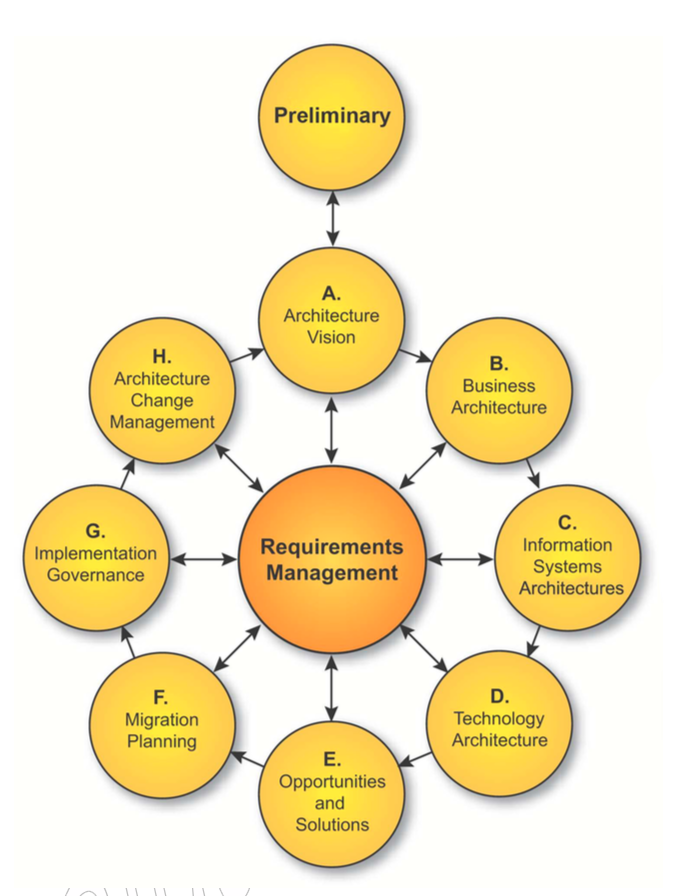
\includegraphics[height=70mm]{images/adm-cycle}
\caption[ADM-Zyklus]{Der ADM-Zyklus \protect\footnotemark}
\label{ADM-Zyklus}
\end{figure}
\footnotetext{Quelle: \cite{TOGAF} S.48 }
\\
Dabei gilt, dass jede Phase einen Output liefert, der als Input für die nächste Phase benutzt wird.\\
Aufgrund des Umfanges werden in dieser Arbeit die Phasen bis C betrachtet. Die konzeptionelle Arbeit wird bis Phase D geleistet, diese wird allerdings ausgeklammert.
\begin{enumerate}
\item{Preliminary}
\\ In der vorgelagerten Phase findet die Eingrenzung des Umfangs auf Basis der Anforderungen statt. 
Ein weiterer Bestandteil ist das ''Tailoring'' statt, in dem das methodische Vorgehen geplant und ggf. gegenüber dem Framework (TOGAF) angepasst wird.\\
Output ist das Dokument ''Request For Architecture Work'', das Ausgangspunkt des Requirement Management ist.
\item{Phase A: Architecture Vision}
\\ In dieser Phase wird richtungsweisend definiert, auf welche Art die zu konzeptionierende Infrastruktur den Anforderungen und Zielen Rechnung tragen soll. Dabei wird auch auf Weiter- oder Wiederverwendungsmöglichkeiten von Bestandsressourcen geschaut.\\
Dies wird in das Dokument''Statement Of Architecture Work'' als Output überführt.
\item{Phase B: Business Architecture}
\\ Phase B definiert die Geschäftsarchitektur hinsichtlich Aufbau- und Ablauforganisation. Das bedeutet, dass hierbei die Anforderungen in konkrete Funktionen und Abläufe überführt werden, was den Output dieser Phase darstellt.
\item{Phase C: Information Systems Architectures}
\\ Die letzte betrachtete Phase definiert die technische Architektur hinsichtlich Datenhaltung und -verarbeitung (Application Architecture). \\
Ein Datenhaltungsmodell und die erforderliche Anwendungs- und Schnittstellenlandschaft werden festgelegt.


\end{enumerate}




\section{Preliminary}
\subsection{Anforderungsanalyse}
\subsubsection{Interne Anforderungen}
\subsubsection{Gesetzliche Anforderungen}

Wird in TOGAF als Preliminary bezeichnet.

\section{Phase A: Architecture Vision}
Phase A Architecture Vision
\section{Phase B: Business Architecutre}
Phase B Business Architecture

\section{Phase C: Information Systems Architectures}
Phase C Information System Architectures

\subsection{Data Architecture}

\subsection{Application Architecture}

\section{Technologieinfrastruktur}